\documentclass[11pt]{IEEEtran}


\usepackage{cite}
\usepackage{amsmath,amssymb,amsfonts}
\usepackage{algorithmic}
\usepackage{graphicx}
\usepackage{textcomp}
\usepackage{xcolor}
\usepackage{pdfpages} 
\def\BibTeX{{\rm B\kern-.05em{\sc i\kern-.025em b}\kern-.08em
  T\kern-.1667em\lower.7ex\hbox{E}\kern-.125emX}}


\begin{document}

\title{EASE MAPE System\\Framework for automatic management of cloud computing resources\\}
\author{
\IEEEauthorblockN{Valentin Laquit}\\
\IEEEauthorblockA{\textit{Intern at Department of Computer Engineering and Software Engineering} \\
\textit{Polytechnique Montreal}\\
 Montreal, Canada \\
 Email: valentin.laquit@gmail.com}
}
\maketitle

\begin{abstract}
 The EASE MAPE System project is a framework design project for the automatic management of IoT resources. It is part of a development process within the EASE group. It is intended to be reused according to different needs. 
 
 The system is based on a MAPE architecture: Monitoring, Analysis, Planning and Execution. The MAPE architecture is in the form of a loop. We can link the IoT application we want to manage.
 
 In order to provide an example of a MAPE loop, the project also contains an implementation for IoT services deployed with Docker Compose. This concrete version of the loop allows you to get some information about the application's performance. Using a threshold comparison algorithm, the MAPE loop is able to size the number of hosting containers.
 
 The system is therefore something extensible and must be implemented according to the use cases.
\end{abstract}
\section{Introduction}
In devops work, automatic management systems (AMS) is a very important aspect of project development. In order to facilitate the development of this type of type of system, and avoid the situation when all the develop of a group create their own little system, it is important to create something extensible and understandable like a framework.

It is in this context that the project has been integrated. Develop a framework based on a MAPE architecture, allowing you to develop your own automatic management system for cloud computing resources.
\subsection{What is a MAPE architecture?}
MAPE is the acronym for \textbf{Monitoring Analysis Planning Execution}.
MAPE loop is a concept introduce by IBM in 2005 to enable an optimized automatic management system for cloud computing resources. 

Concretely the loop will automatically manage the system by connecting to the client application or system, monitor, analyze, plan and execute adaptive action.
 
In our case it will follow something like the following diagram:
\begin{figure}[h]
\centerline{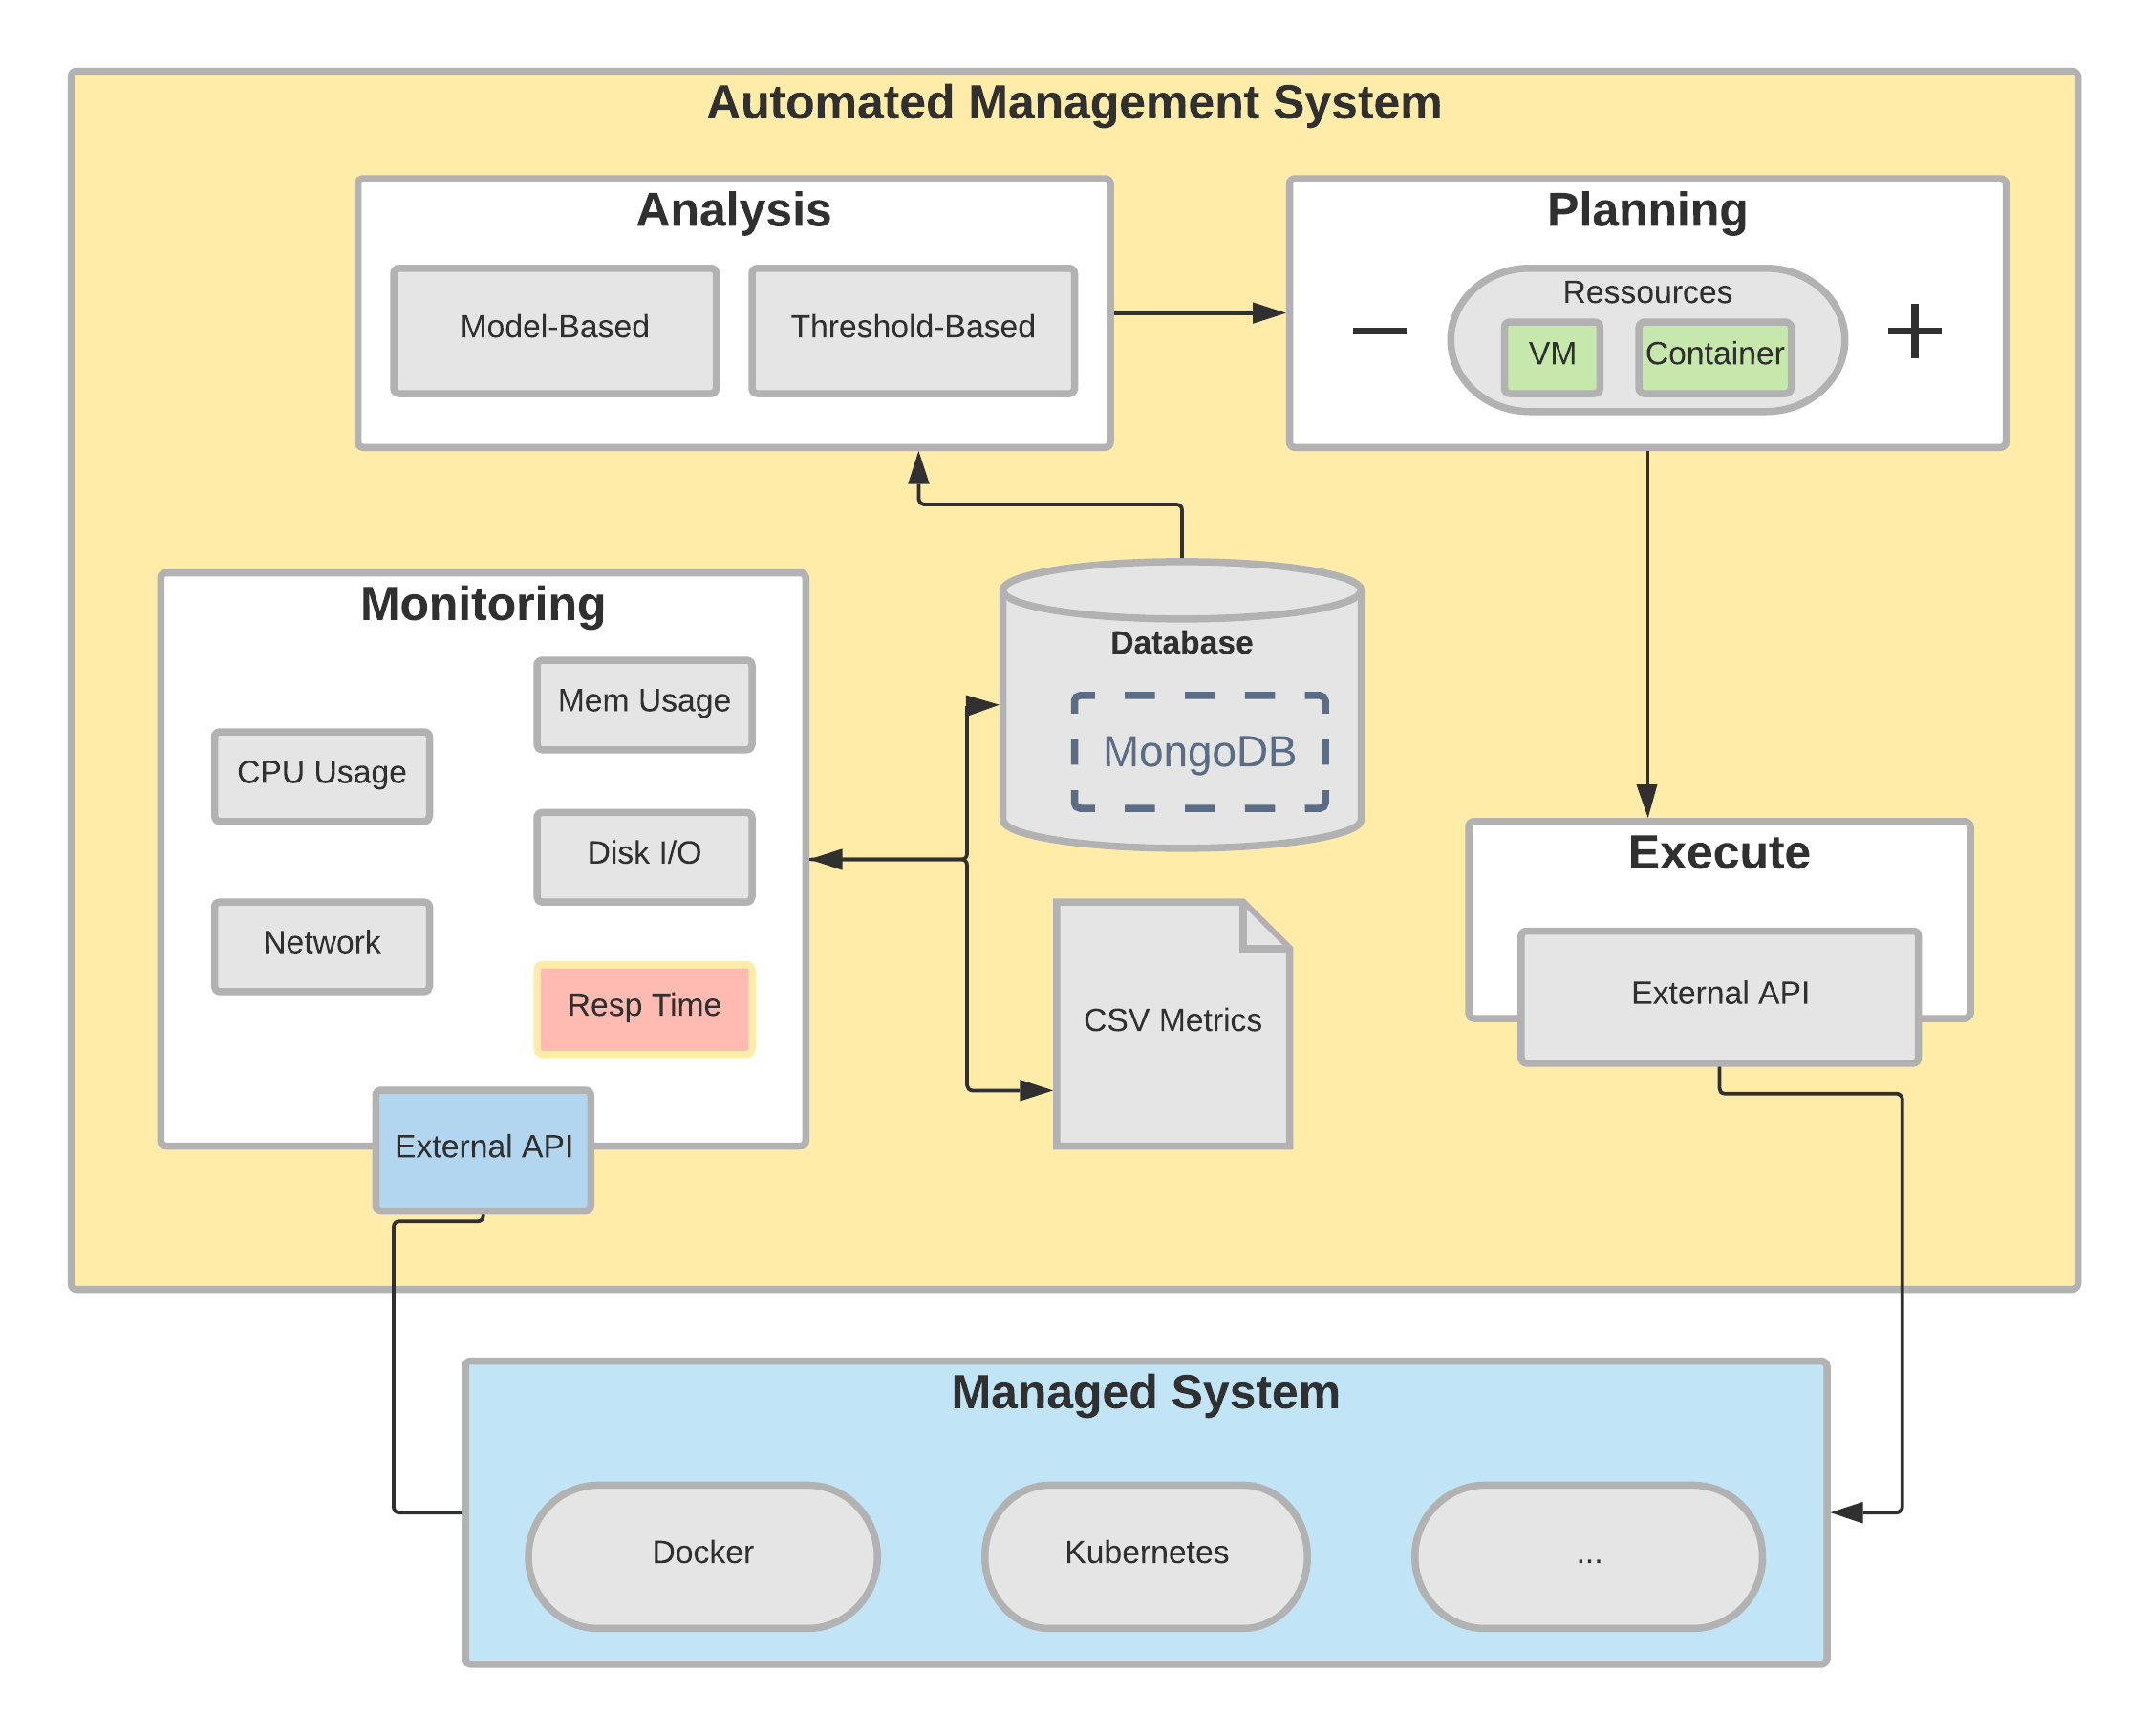
\includegraphics[width=\linewidth]{mape_diagram.png}}
\caption{EASE MAPE System architecture}
\label{fig}
\end{figure}

\subsection{Framework components}
\begin{itemize}
\item \textbf{Monitoring}\\
Monitoring needs to be connected to a client (like docker environment) and
a database. It is supposed to get different data from the client like CPU, memory, disks I/O and network throughput of components, and store them into the NoSQL database in JSON document format. It can also get and store current date and for example the number of containers running on the client. 

The main point is that the monitoring needs to run independently of the other modules. Because if something happens in other parts of the system the monitoring should continue to get information from the client.

\item \textbf{Analysis}\\
Analysis needs to be connected to the database because he will periodically read the new information stored. Because of the threshold-based used in our experiments, the analysis module should concentrate his analyze on the CPU and compare it with the threshold of our choice. It should return a list of information to the planning module. But the analysis can implement any type of model, corresponding to user needs.

\item \textbf{Planning}\\
Planning is a bit similar to the analysis but he only has to get information from analysis and plan the adaptive action. For example, add or remove containers in the case of Docker monitoring. And then send the decision to the execution module.

\item \textbf{Execution}\\
The execution module receives decisions from the planning module and execute the decision. He has to use the corresponding API and make a break in the MAPE loop until the system stability is reached. 

\end{itemize}

\section{Development process}
\subsection{Goal and constraint}
1. The main goal of this project was to build a framework. Being a framework, we want the components of Monitoring, Analysis, Planning, Execution need to be extendable to allow for plugging services from external providers. More specifically, the framework components need to be abstract and simply define an interface to access the functionality of the individual component. 

2. Secondly, we had to provide a concrete Docker implementation with Docker Compose scaling. This implementation will provide a "guideline" for the development.

3. The second point was to provide a complete user manual. Because the system is a framework, the manual should contain a development guideline. But it must contain the tutorial for running the existing implementation.

\subsection{Tools}
\textbf{Pycharm:} 
PyCharm is a JetBrain Company IDE that allows a lot things in Python projects. This was a very powerful IDE  to develop this project because it allows us to run different programs and debug them. It is also connected to GitHub in order to commit modifications.

It provides auto completion, code refactorings, inspections, error highlighting and quick fixes. \\

\textbf{MongoDB:}
MongoDB is a general purpose, document-based, distributed NoSQL database. MongoDB is a document database, which means it stores data in JSON-like documents. It is very useful when you need to store data with lots of information like a monitoring algorithm can do.

In our work it was very simple to use this database because it can be built locally with containers. The query in Python with Pymongo modules are very easy to understand. \\


\textbf{Docker:}
Docker is the well know container services that provide a lot of functionality for running containers.This is a very large service used everywhere. 

Then in our case we used docker to deploy test application of IoT simulation and database deployment. There is multiple way to interact with docker containers, but the remote API is a pretty good way because it provides JSON information.

The main point is that to have a deployment service, you cannot run containers independently. That why we used Docker Compose, to run multiple containers.\\

\textbf{Docker Compose:}
As mentionned just below, Docker Compose is a tool for defining and running multi-container Docker applications. 

"With Compose, you use a YAML file to configure your application’s services. Then, with a single command, you create and start all the services from your configuration." \cite{b1}

We used docker compose to deploy the test app and also to scale our application with the command line.\\


\textbf{PyBuilder:}
"PyBuilder is a software build tool written in pure Python which mainly targets Python applications. It is based on the concept of dependency based programming but also comes along with a powerful plugin mechanism that allows the construction of build life cycles similar to those known from other famous build tools like Apache Maven."\cite{b2}

Pybluider was integrated in the project in order to installs dependencies automatically by using this build tool.\\

\textbf{PowerAPI:}
PowerAPI is a tool under development to estimate the energy consumption of a machine. More specifically, the CPU usage.

We used PowerAPI to provide us with one more data to monitor. Energy consumption in Watt.

This can allow, for example, to provide an analysis based on something other than just use in %.


\section{Docker client implementation}
In order to provide a concrete version of the MAPE loop, we decided to implement a Docker client management system. 

This concrete version will help developers to implement their own version of the loop by following the framework and get inspired by the existing one.

\subsection{Docker remote API}
Docker is a service which provides a lot of possibilities. As a lot of services he gives access to a Rest API. This API is available in multiple languages, and in our case the Python one is what we needed. 


\subsection{CPU threshold analysis}
The threshold analysis method is the easiest way to manage the CPU utilization. 

The thresholds are defined in the configuration file based on the needs of the user. The analysis algorithm is connected to the database where the monitoring data are stored. It will query the database every 10 seconde for example and compare the CPU of this last information with the thresholds. If something CPU reached one of the thresholds, the analysis method will call the planning part.

This planning part is nearly the same as the analysis part but it will decide how many containers to scale. Just after the decision is taken, the planning algorithm call the execution and then the execution execute the decision by calling bash command.

\section{Experiments}
After developing the Docker concrete implementation, it was necessary to test it with a complete simulation of Docker environment with workload generators.
\subsection{Using IoT sensors simulation}
To test the application we used an IoT simulation. This simulation is launched with Docker Compose. When you run the Docker Compose command there are multiple services starting: 
\begin{itemize}
 \item Local MongoDB database
 \item HAproxy, proxy to load balance requests
 \item Web services container to receive requests
 \item IoT simulator to provide a scheduled number of requests per second
\end{itemize}
So the container to monitor is the web container because this is the one who receives the more request and he is likely to receive the most requests.
\subsection{Results}
So when the MAPE loop is connected to the docker environment where the IoT simulation is running, we could expect the autoscale working. 

Here is an example of a simulation:
\begin{figure}[h]
 \centerline{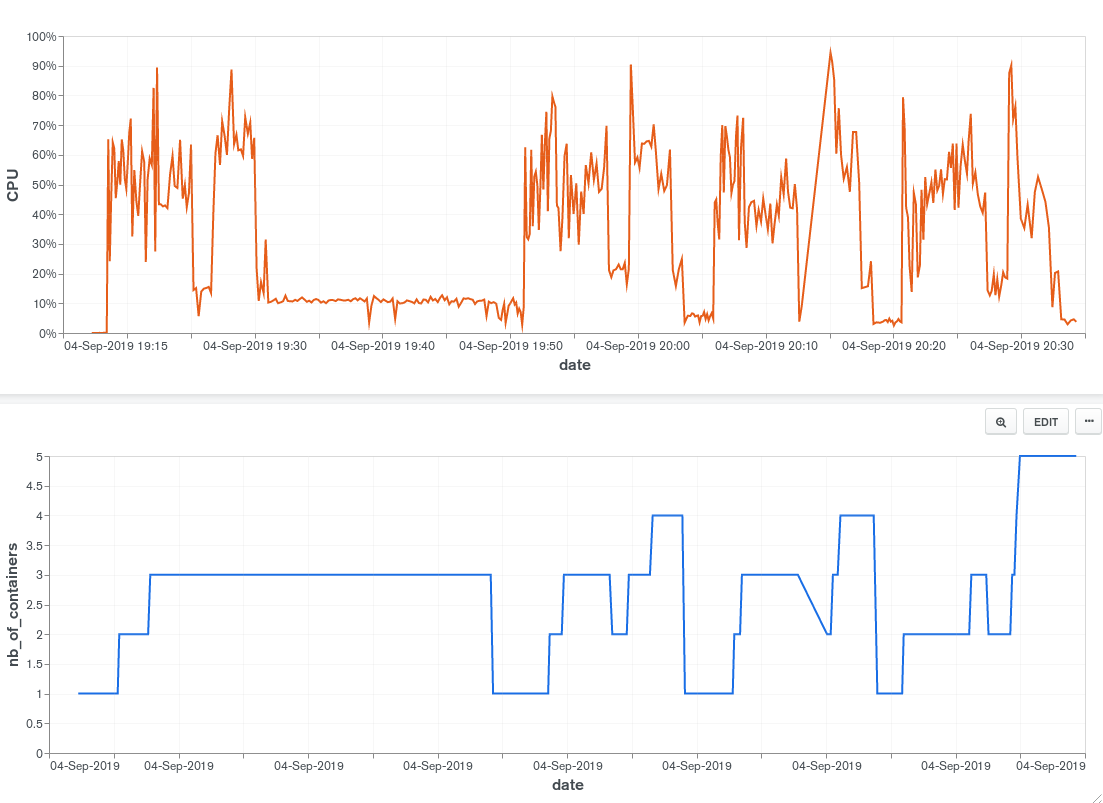
\includegraphics[width=\linewidth]{threshold.png}}
 \caption{Evolution of CPU utilization and a number of containers for the web service}
\end{figure}

As we can see, in orange we have the CPU utilization for the web service and the blue represent the number of containers.The threshold was fixed to 60\% upper and 15\% lower. It is not the most optimal thresholds but this is correct for the experiment. 

The number of containers is not scaling every time the CPU is reaching one the threshold because the analysis takes a short section of time can calculate an average of the CPU utilization. That why sometime nothing appends.

Another example of thresholds autoscaling:
\begin{figure}[h]
 \centerline{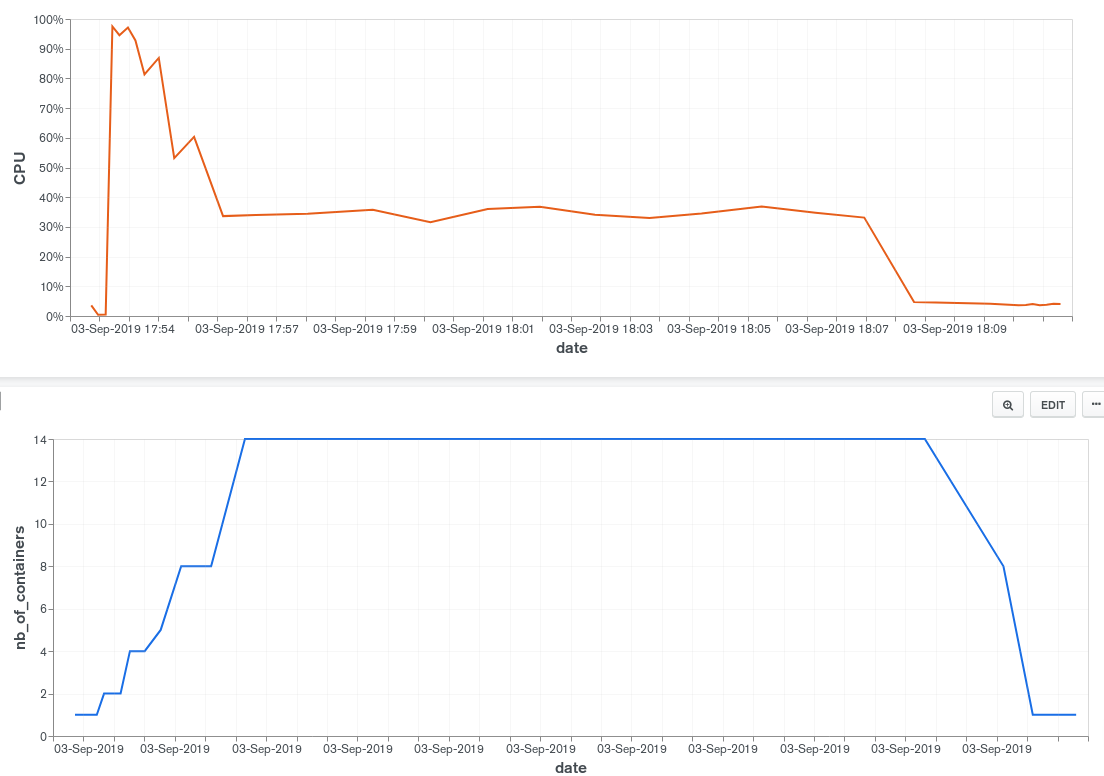
\includegraphics[width=\linewidth]{diagram_smoothed.png}}
 \caption{Evolution of CPU utilization and a number of containers smoothed}
\end{figure}

This result seems much more satisfying. Indeed, the analysis algorithm has been modified in order to compare the last 5 CPU values in order not to cause a bounce. 
This results in a much more stable container auto scale.  

\section{Conclusion}
This work has therefore led to several things. 
First of all, the idea of providing an extensible framework to be reused was reached. Indeed, a guideline has been defined in order to have a basis in the development of an automatic management system. 

Secondly, the objective of providing an implementation example by following the framework was also achieved. There is therefore an implementation for the Docker environment that can be used as a guide.

Then, since the project will have to be further developed, the documentation provided had to allow this. This documentation therefore includes a tutorial and a user manual to build your own version of the MAPE loop.

In the future the objective is to continue to improve the framework, and to provide new versions of automatic management via different analysis algorithms, for example.


\section*{Acknowledgment}
Thank you to Marios Fokaefs, teacher researchers at Polytechnique Montreal, for bringing the idea for this project to us. To have supervised, reviewed and ensured the credibility of the work provided. 

Thanks to MohammadReza Rasol, for collaborating in the design and testing of the framework.

\begin{thebibliography}{00}
 \bibitem{b1} 
 https://docs.docker.com/compose/
 \bibitem{b2}
 http://pybuilder.github.io/
\end{thebibliography}

\newpage
\appendices
\section{User manual}
\label{User manual}
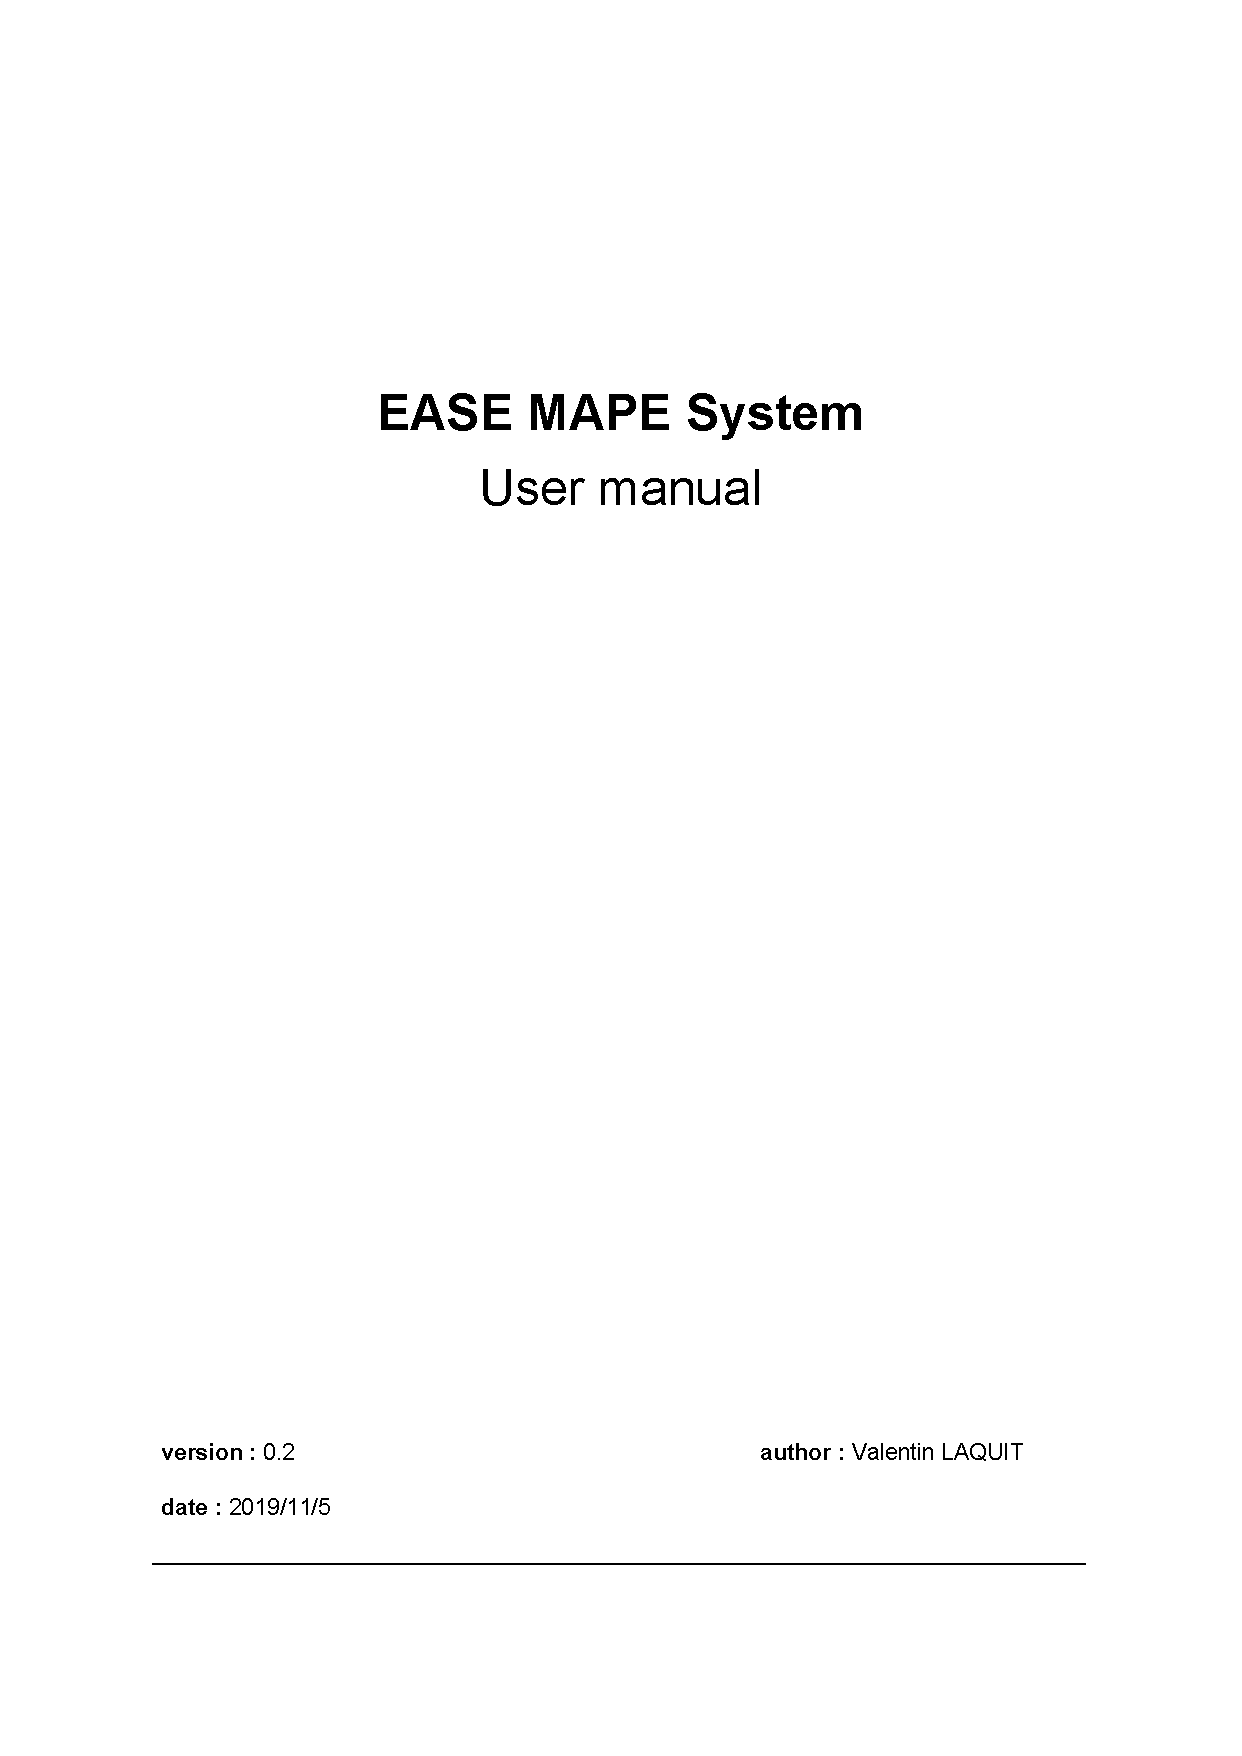
\includepdf[page=-]{usersmanual.pdf}

\end{document}
